\section{Methods}

% \subsection{LCS-based frame wise alignment}

% % \begin{figure}[ht]
% %     \centering
% %     \includegraphics[height=10.5cm]{figure/Cost_Prediction.png}
% %     \caption{Comparison of Time-based and Token-based Methods}
% %     \label{method-comparison}
% % \end{figure}

% In this part, we propose a novel method for frame wise speech-text alignment based on LCS(Longest Common Sequence) algorithm, unlike existing methods for forced alignment which strictly requires that each frame has a corresponding text token. 
% Our method only aligns certain frames and text tokens with high matching scores. We will explain the matching scores in \ref{alg1}.

% \begin{algorithm}
% \caption{LCS-based Sequence Alignment}\label{alg1}
% \footnotesize
% \begin{algorithmic}[1]
% \Statex \textbf{Input:} 
%     $Label$ (phoneme labels), 
%     $Time$ (time frames), 
%     $C$ (cost matrix), 
%     $tol$ (tolerance),
%     $phn\_sim$ (similarity dictionary)
% \Statex \textbf{Output:} Alignment path or mask

% \Procedure{Align}{$Label$, $Time$, $C$, $tol$, $phn\_sim$}
%     \State $valid\_res \gets \emptyset$
%     \For{$(i,j) \in [0,n) \times [0,m)$}
%         \State $phn1 \gets Label[i]$, $phn2 \gets Label[k]$ \Comment{$k=\arg\min C[:,j]$}
%         \State $sim \gets phn\_sim[(phn1,phn2)]$ \Comment{Lookup similarity}
%         \If{$C[i][j] \leq (1-sim) \times tol$} \Comment{Similarity-adjusted threshold}
%             \State $valid\_res \gets valid\_res \cup \{(i,j), (j,i)\}$
%         \EndIf
%     \EndFor
    
%     \State $dp \gets \text{zeros}(n+1,m+1)$
%     \For{$i \gets 1$ to $n$}
%         \For{$j \gets 1$ to $m$}
%             \If{$(i-1,j-1) \in valid\_res$}
%                 \State $dp[i][j] \gets \max(dp[i-1][j-1]+1, dp[i][j-1])$
%                 \For{$k \gets j+1$ to $m$} \Comment{Propagate valid matches}
%                     \State $dp[i][k] \gets dp[i][k-1] + \mathbb{I}_{(i-1,k-1) \in valid\_res}$
%                 \EndFor
%             \Else
%                 \State $dp[i][j] \gets \max(dp[i-1][j], dp[i][j-1])$
%             \EndIf
%         \EndFor
%     \EndFor
    
%     \State \Return $\text{MaskFromPath}(\text{Traceback}(dp))$
% \EndProcedure
% \end{algorithmic}
% \end{algorithm}

% The proposed phoneme-aware LCS alignment algorithm dynamically adapts to phonetic similarity patterns through a multi-stage process. First, it identifies valid frame-label pairs $(i,j)$ by comparing the cost matrix entries $C[i,j]$ against similarity-adjusted thresholds $(1-s(phn_i,phn_k))\cdot tol$, where $s(phn_i,phn_k)$ is retrieved from a pre-trained phonetic similarity dictionary $phn\_sim$. This adaptive thresholding relaxes alignment constraints for acoustically similar phoneme pairs while maintaining strict boundaries for dissimilar ones. The algorithm then constructs a dynamic programming table $dp$ where each entry $dp[i][j]$ maximizes the alignment path continuity through three possible moves: diagonal (matched pair), vertical (label skip), or horizontal (frame skip). Notably, when valid matches are detected, the solution propagates horizontally to preserve sequential alignment continuity. Finally, the traceback procedure extracts either an alignment path $\mathcal{P} = \{(i_t,j_t)\}_{t=1}^T$ and generates a binary mask matrix $M \in \{0,1\}^{n \times m}$ where $M[i,j] = 1$ indicates aligned pairs. This dual-output design supports both traditional ASR pipeline integration and neural network training, with the phonetic similarity integration particularly effective for confusable phoneme sequences in noisy conditions.
\begin{figure}[t]
    \centering
    \begin{subfigure}{\columnwidth}
        \centering
        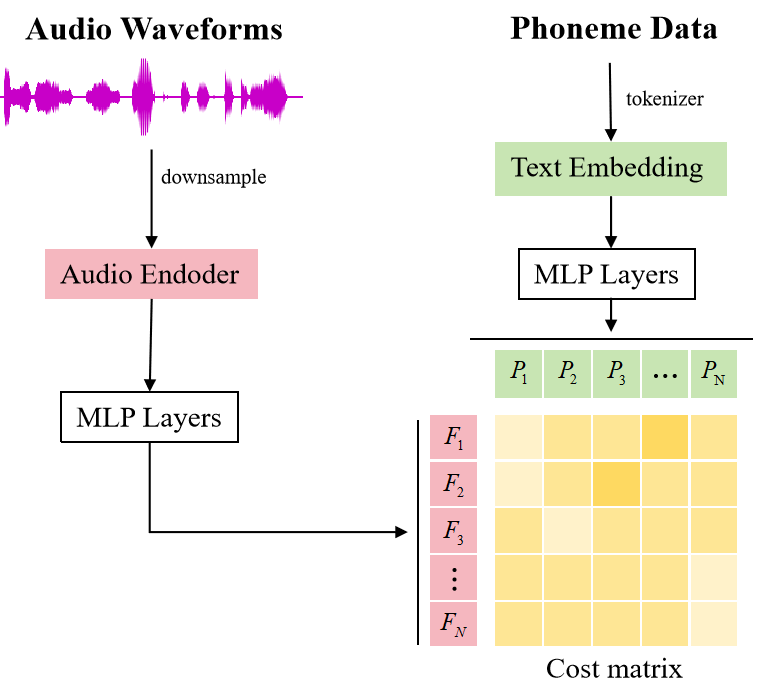
\includegraphics[width=0.9\textwidth]{figure/cost.png}
        \caption{}
        \label{fig:sub1}
    \end{subfigure}
    
    \vspace{1em}
    \begin{subfigure}{\columnwidth}
        \centering
        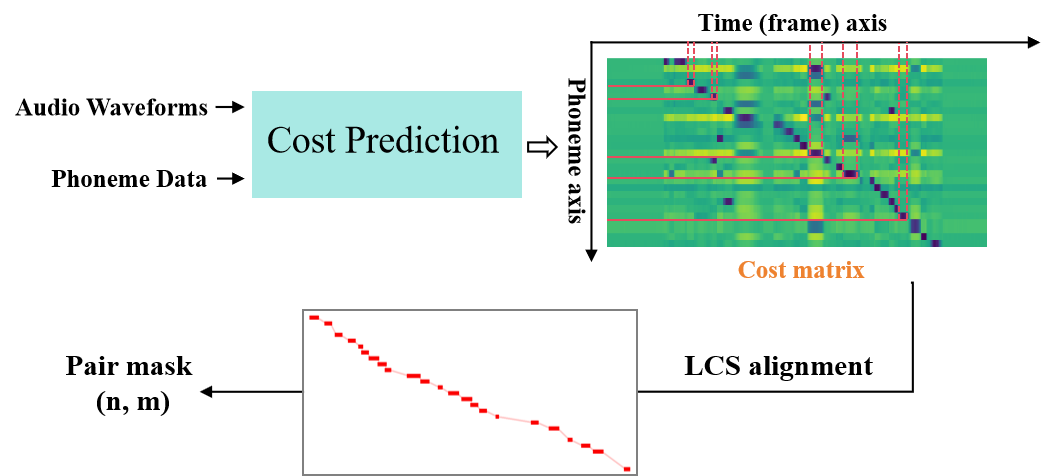
\includegraphics[width=1.0\textwidth]{figure/aligner.png}
        \caption{}
        \label{fig:sub2}
    \end{subfigure}
    
    \caption{(a) shows the structure of cost matrix learning model. (b) shows the process from predicted cost matrix to alignment mask: we use cost matrix to construct the dynamic programming matrix and implement modified LCS algorithm to realize a local wise alignment, the dark red dots indicate credible local alignment regions.}
    \label{fig:combined}
    \vspace{-1.8em}
\end{figure}

\begin{figure*}[t]
  \centering
  
\includegraphics[width=0.8\textwidth]{figure/pipeline.png}
  \caption{\textit{Overview of LCS-CTC framework}: (a) Vanilla CTC allows all valid alignment paths that collapse to the target sequence, which can result in peaky distributions.  
(b) Our LCS-CTC introduces alignment constraints from the LCS-based aligner (black nodes), which eliminate implausible paths (red crosses) by fixing "high-confidence" frame-phoneme matches.  
(c) The overall training pipeline of LCS-CTC. The LCS aligner uses ground-truth phonemes and predicted emissions to generate alignment masks, which are then used both as supervision (via $\mathcal{L}_{\text{CE}}$) and constraint (via masked $\mathcal{L}_{\text{CTC}}$) during recognition model training.}
  \label{fig:pipeline}
      \vspace{-11pt}
\end{figure*}

\begin{algorithm}[h]
\caption{LCS-based Sequence Alignment}\label{alg1}
\footnotesize
\begin{algorithmic}[1]
\Statex \textbf{Input:} 
    $Label$ (phoneme labels), 
    $C$ (cost matrix), 
    $tol$ (tolerance),
    $phn\_sim$ (similarity dictionary)
\Statex \textbf{Output:} Alignment mask

\Procedure{Align}{$Label$, $C$, $tol$, $phn\_sim$}
    \State $valid\_res \gets \emptyset$
    \For{$(i,j) \in [0,n) \times [0,m)$}
        \State $phn1 \gets Label[i]$, $phn2 \gets Label[k]$ \Comment{$k=\arg\min C[:,j]$}
        \State $sim \gets phn\_sim[(phn1,phn2)]$ \Comment{Lookup similarity}
        \If{$C[i][j] \leq (1-sim) \times tol$} \Comment{Similarity-adjusted threshold}
            \State $valid\_res \gets valid\_res \cup \{(i,j), (j,i)\}$
        \EndIf
    \EndFor
    
    \State $dp \gets \text{zeros}(n+1,m+1)$
    \For{$i \gets 1$ to $n$}
        \For{$j \gets 1$ to $m$}
            \If{$(i-1,j-1) \in valid\_res$}
                \State $dp[i][j] \gets \max(dp[i-1][j-1]+1, dp[i][j-1])$
                \For{$k \gets j+1$ to $m$} \Comment{Propagate valid matches}
                    \State $dp[i][k] \gets dp[i][k-1] + \mathbb{I}_{(i-1,k-1) \in valid\_res}$
                \EndFor
\Statex \quad The indicator function $\mathbb{I}_{(i{-}1,k{-}1) \in \textit{valid\_res}}$ ensures that alignment credit is propagated horizontally across frames that are all considered valid matches to phoneme $i{-}1$.
            \Else
                \State $dp[i][j] \gets \max(dp[i-1][j], dp[i][j-1])$
            \EndIf
        \EndFor
    \EndFor

    \State $path \gets$ \Call{Traceback}{$dp$} \Comment{Recover alignment path from DP}
    \State \Return $\text{MaskFromPath}(path)$
\EndProcedure
\end{algorithmic}
\end{algorithm}

The LCS-CTC framework comprises two stages: local alignment extraction via similarity-aware LCS, and constrained CTC training using the resulting alignment masks. This design aims to improve ASR robustness by enforcing phonemically plausible supervision while preserving temporal flexibility.

\subsection{Similarity-Guided LCS Alignment}
\label{sec:lcs-align}

In this section, we propose a novel method for frame-wise speech-text alignment inspired by the Longest Common Subsequence (LCS) algorithm~\cite{hirschberg1977algorithms-lcs1}. Unlike traditional forced alignment approaches that enforce strict one-to-one alignment between each speech frame and a corresponding phoneme label, our method relaxes this assumption by focusing only on “highly confident" frame-label pairs. This partial alignment strategy better reflects the acoustic variability in natural speech, such as ambiguous onsets and offsets, where the phonetic boundaries are inherently fuzzy.

\paragraph{Overview} Our method consists of two key stages: (1) predicting a fine-grained cost matrix between speech frames and phoneme labels using a neural model, and (2) applying a similarity-aware dynamic programming alignment inspired by LCS. The goal is to identify optimal frame-label matches that reflect both acoustic evidence and phonetic similarity. The process of our method is shown in Fig.~\ref{fig:combined}

\paragraph{Cost Matrix Learning} Given a speech utterance segmented into $m$ frames and its corresponding phoneme sequence of length $n$, we train a neural model to predict a cost matrix $C \in \mathbb{R}^{n \times m}$ where $C[i,j]$ estimates the alignment cost between the $i$-th phoneme and the $j$-th frame. The model is trained using a subset of VCTK~\cite{yamagishi2019cstr-vctk} data, for which accurate frame-level alignments are obtained via Montreal Forced Aligner (MFA)~\cite{mcauliffe17_interspeech} and manually corrected annotations.


To construct target labels for supervision, we incorporate a pre-defined phoneme similarity function $s: \mathcal{P_\text{cmu}} \times \mathcal{P_\text{cmu}} \rightarrow [0,1]$, where $\mathcal{P_\text{cmu}}$ denotes the set of CMU phonemes. This similarity is computed based on a set of eight articulatory features, including phoneme type (vowel/consonant), vowel length, height, frontness, lip rounding, consonant manner, place of articulation, and voicing. Let the ground-truth aligned phoneme for frame $t_j$ be $p^*_j$; then the target cost for matching phoneme $p_i$ to frame $t_j$ is defined as:
\[
\tilde{C}[i,j] =
\begin{cases}
0, & \text{if } p_i = p^*_j, \\
1 - s(p_i, p^*_j), & \text{otherwise}.
\end{cases}
\]

To account for temporal uncertainty at phoneme boundaries (e.g., transitional blur at start or end of a phoneme), we further apply a Gaussian edge attenuation to the ground-truth aligned region.Finally, the cost matrix labels $\tilde{C}$ are normalized across the time axis via softmax. For convenience, we denote $s(p_i,p_j)$ as the similarity values after softmax.

To learn this cost matrix label, we design a model that jointly encodes both the audio signal and the target phoneme sequence. The audio input is first passed through a pretrained audio encoder (e.g., Wav2Vec2~\cite{baevski2020wav2vec20frameworkselfsupervised}), producing a sequence of frame-level acoustic embeddings. Simultaneously, the phoneme sequence is mapped into dense embeddings. Each of the two modalities is then processed by separate MLPs to project them into a shared hidden space. The projected frame and phoneme features are combined via negative dot product, followed by a softmax over the time axis. The resulting matrix is then trained to match the cost matrix labels using a Kullback-Leibler (KL) divergence loss. The structure of the model is illustrated in Fig.~\ref{fig:sub1}.

\paragraph{Similarity-Aware LCS Alignment} Once the model yields a predicted cost matrix $C$, we proceed to perform a similarity-informed dynamic alignment. The alignment algorithm identifies all phoneme-frame pairs $(i,j)$ which the predicted cost $C[i,j]$ falls below a similarity-adjusted threshold $\tau_{i,j} = (1 - s(p_i, p_j)) \cdot \text{tol}$, where $\text{tol}$ is a global tolerance hyperparameter, and we set tol = 1 in our work, the selection process is shown in Section~\ref{abl}. This yields a set of valid match candidates:
\[
\begin{aligned}
valid\_res &= \{(i,j) \mid C[i,j] \leq (1 - s(p_i, p_k)) \cdot \text{tol}\}, \\
&\quad \text{with } k = \arg\min_{i} C[i,j].
\end{aligned}
\]

The implementation of the algorithm is shown in Algorithm~\ref{alg1}. It outputs binary alignment mask $M^{'} \in \{0,1\}^{n \times m}$ derived from the alignment path where $M^{'}[i,j] = 1$ if phoneme $p_i$ aligns with frame $t_j$. This design allows integration into traditional ASR pipelines which we will talk below.

By integrating phonetic similarity into the cost prediction and alignment stages, our method enables more robust alignment in the presence of acoustic ambiguity or phoneme confusability. The process from cost matrix to alignment mask can be seen in Fig.~\ref{fig:sub2}.

\subsection{Constrained LCS-CTC for ASR Training}


\subsubsection{Review on Connectionist Temporal Classification (CTC)}

The CTC loss has been widely adopted in ASR systems for its ability to model frame-to-label alignments with length mismatch. Given an input sequence of acoustic features $X = \{x_1, x_2, \dots, x_T\}$ and a target label sequence $Y = \{y_1, y_2, \dots, y_L\}$, CTC computes the loss by marginalizing over all possible frame-to-label alignments $\pi \in \mathcal{B}^{-1}(Y)$ where $\mathcal{B}$ is the many-to-one mapping function that removes blank tokens and repeated labels. Vanilla CTC loss is defined as:

\begin{equation*}
\mathcal{L}_{\text{CTC}} = -\log \sum_{\pi \in \mathcal{B}^{-1}(Y)} P(\pi \mid X)
\end{equation*}

 While flexible, vanilla CTC suffers from the \emph{peaky distribution} problem, where probability mass tends to concentrate on a few frames, leading to unreliable and non-robust alignments. Moreover, it treats all frame-label alignments as equally likely during training, regardless of their phonetic plausibility, which can harm generalization in downstream recognition tasks.

\subsubsection{LCS-CTC: Constrained CTC Training with Alignment Masks}


To enhance the robustness and generalization ability of the recognition model trained by CTC, we propose a novel CTC variant named \textbf{LCS-CTC}, which integrates frame-phoneme alignment masks derived from similarity-aware LCS algorithm (as introduced in Section~\ref{sec:lcs-align}). The central idea is to apply the LCS-derived alignment mask as a constraint over the CTC emission probabilities, thereby pruning unlikely frame-to-phoneme associations during training. In our recognition model, the input audio signal is first encoded by a pretrained speech encoder, followed by a stack of 8 Conformer layers~\cite{gulati2020conformer} and an MLP-based classifier head that produces the final emission probabilities. Since the emission matrix $P \in \mathbb{R}^{L \times T}$ represents the frame-wise posterior over the entire phoneme vocabulary $\mathcal{P_\text{cmu}}$ of size $L$, we transform the original alignment mask $M^{'}$(of shape $n \times T$ for a target sequence of length $n$) into a binary matrix $M \in \{0,1\}^{L \times T}$, where $M[i,j] = 1$ indicates that frame $t_j$ is constrained to emit phoneme $p_i$. This transformation ensures compatibility between the alignment constraint and the CTC output space.

The masked emission $\tilde{P}$ is computed by applying the alignment mask $M$ to the original CTC emission $P$:

% \begin{equation*}
% \tilde{P}[i,j] = \frac{P[i,j] \cdot M[i,j]  + \epsilon}{\sum_{k} P[i,k] \cdot M[i,k]}
% \end{equation*}

\begin{equation*}
\tilde{P}[i,j] =
\begin{cases}
\displaystyle\frac{P[i,j] \cdot M[i,j] + \epsilon}{\sum_{l} P[l,j] \cdot M[l,j] + \epsilon}, & \text{if } \sum_{l} M[l,j] > 0 \\
P[i,j], & \text{otherwise}
\end{cases}
\end{equation*}


where $\epsilon$ is a small constant to ensure numerical stability. This operation selectively normalizes emission probabilities at frames that are constrained by the LCS-derived alignment mask, while leaving unconstrained frames unchanged. 

We then define a hybrid training objective that supervises the model in two complementary ways. First, for the high-confidence alignment regions specified by the binary mask $M$, we apply cross-entropy loss directly on the original emission $P$ to provide strong local supervision. Second, we apply vanilla CTC loss over the full sequence using the masked emission $\tilde{P}$, which softly restricts the CTC decoding space during sequence-level training. Crucially, by anchoring certain frames to fixed phoneme labels through $M$, our method effectively eliminates implausible alignment paths and narrows the search space, thereby improving CTC training stability and generalization. The details are illustrated in Fig.~\ref{fig:pipeline}.


The final loss is computed as:
\begin{equation*}
\mathcal{L}_{\text{LCS-CTC}} = \lambda \cdot \mathcal{L}_{\text{CE}}(P \odot M, Y) + (1 - \lambda) \cdot \mathcal{L}_{\text{CTC}}(\tilde{P}, Y)
\end{equation*}

where $\odot$ denotes element-wise masking. Here, $\mathcal{L}_{\text{CE}}$ denotes standard cross-entropy loss evaluated only on masked positions, while $\lambda \in [0,1]$ is a weighting factor balancing between strict alignment enforcement and flexible CTC decoding. We set $\lambda = 0.5$ in our work. This hybrid objective ensures that the model is supervised on phonemically plausible alignments while retaining the benefits of sequence-level flexibility.

